\section{Functional Partitioning}

\begin{content}
  ECAP5-DPROC is built around a pipelined architecture with the following stages :
  \begin{itemize}
    \vspace{-0.5em}
    \item The instruction fetch stage loads the next instruction from memory.
    \vspace{-0.5em}
    \item The decode stage handles the instruction decoding to provide the next stage with the different instruction input values including reading from internal registers.
    \vspace{-0.5em}
    \item The execute stage implements instruction behaviors. This includes performing integer operations as well as accessing memory.
    \vspace{-0.5em}
    \item The write-back stage which handles storing instructions outputs to internal registers.
  \end{itemize}

\begin{figure}[h!]
    \centering
    \vspace{1em}
\scalebox{0.75}{
\begin{tikzpicture}[scale=1.25, draw=gray, inner sep=0, outer sep=0]
  \node[rectangle, draw=black,
    minimum height = 1.25cm,
    minimum width = 10cm,
    fill = gray!20] (EMM) at (6, -2.5) {EMM};
  \node[rectangle, draw=black,
    minimum height = 2cm,
    minimum width = 2cm,
    fill = blue!20!gray!20] (IFM) at (3, 0) {IFM};
  \node[rectangle, draw=black,
    minimum height = 2cm,
    minimum width = 2cm,
    fill = blue!20!gray!20] (DECM) at (6, 0) {DECM};
  \node[rectangle, draw=black,
    minimum height = 1.25cm,
    minimum width = 10cm,
    fill = gray!20] (REGM) at (9, 2.5) {REGM};
  \node[rectangle, draw=black,
    minimum height = 2cm,
    minimum width = 2cm,
    fill = blue!20!gray!20] (EXM) at (9, 0) {EXM};
  \node[rectangle, draw=black,
    minimum height = 2cm,
    minimum width = 2cm,
    fill = blue!20!gray!20] (WBM) at (12, 0) {WBM};

  \draw[->] (IFM.east) -- (DECM.west);
  \draw[->] (DECM.east) -- (EXM.west);
  \draw[->] (EXM.east) -- (WBM.west);

  \draw[<-] (IFM.south) -- (IFM.south|- EMM.north);

  \draw[->] ([xshift=-0.25cm]EXM.south) -- ([xshift=-0.25cm]EXM.south |- EMM.north);
  \draw[<-] ([xshift=0.25cm]EXM.south) -- ([xshift=0.25cm]EXM.south |- EMM.north);

  \draw[<-] (DECM.north) -- (DECM.north |- REGM.south);
  \draw[->] (WBM.north) -- (WBM.north |- REGM.south);

  % surrounding rectangle
  \node[dashed, draw=black, align=center, inner sep=0.5cm, fit=(EMM) (IFM) (DECM) (EXM) (WBM) (REGM)] (border) {};
  \node[anchor=north west, inner sep=0.5cm] (border-text) at (border.north west) {TOPM};

  % external interface
  \node (irq) at ([yshift=0.25cm]IFM.west) {};
  \node (drq) at ([yshift=-0.25cm]IFM.west) {};
  \node (axi) at (EMM.west) {};
  \node (clk) at ([yshift=-1.25cm]border.north west) {};
  \node (rst) at ([yshift=-1.75cm]border.north west) {};

  \node (extend) at ([xshift=-1.5cm]irq.center) {};

  \draw[->] (clk.center -| extend.center) node[left=0.2cm, anchor=east]{\small CLK} -- (clk.center);
  \draw[->] (rst.center -| extend.center) node[left=0.2cm, anchor=east]{\small RST\_N} -- (rst.center);
  \draw[->] (irq.center -| extend.center) node[left=0.2cm, anchor=east]{\small IRQ} -- (irq.center);
  \draw[->] (drq.center -| extend.center) node[left=0.2cm, anchor=east]{\small DRQ} -- (drq.center);
  \draw[<->, thick] (axi.center -| extend.center) node[left=0.2cm, anchor=east]{\small AXI-Lite} -- (axi.center);

  % clk triangle
  \draw[-, dashed] ([yshift=0.25cm]clk.center) -- ([xshift=0.25cm]clk.center) -- ([yshift=-0.25cm]clk.center);

\end{tikzpicture}
}

    \caption{Schematic view of the architecture of ECAP5-DPROC}
    \label{fig:architecture}
\end{figure}

  The design is split into the following functional modules :
  \begin{itemize}
    \vspace{-0.5em}
    \item The \textbf{Top Module} (TOPM) which integrates all other modules.
    \item The \textbf{External Memory Module} (EMM), in charge of accessing memory and peripherals.
    \vspace{-0.5em}
    \item The \textbf{Instruction Fetch Module} (IFM), in charge of implementing the instruction fetch stage.
    \vspace{-0.5em}
    \item The \textbf{Decode Module} (DECM), in charge of implementing the decode stage.
    \vspace{-0.5em}
    \item The \textbf{Register Module} (REGM), implementing the internal registers.
    \vspace{-0.5em}
    \item The \textbf{Execute Module} (EXM), in charge of implementing the execute stage.
    \item The \textbf{Write-Back Module} (WBM), in charge of implementing the write-back stage.
  \end{itemize}
\end{content}

\newpage

\section{Top Module}

\begin{content}
  Handshaking and bubbling
\end{content}

\newpage

\section{External Memory Module}
\newpage

\section{Instruction Fetch Module}
\begin{figure}[h!]
    \centering
    \vspace{1em}
\scalebox{0.85}{
\begin{tikzpicture}[scale=1.25, draw=gray, inner sep=0, outer sep=0]
  \node[rectangle, draw=white,
    minimum height = 5cm,
    minimum width = 2cm] (back) at (0, 0) {};
  \node[rectangle, draw=black,
    anchor=south,
    align=center,
    minimum height = 4.5cm,
    minimum width = 2.5cm,
    fill = gray!20] (mem) at (back.south) {Memory\\read};
  \node[rectangle, draw=black,
    align=center,
    anchor=north east,
    minimum height = 0.75cm,
    minimum width = 2cm,
    fill = blue!20!gray!20] (pc) at ([xshift=-1cm]mem.north west) {pc};
  \node[rectangle, draw=black,
    align=center,
    anchor=south east,
    minimum height = 3cm,
    minimum width = 2cm,
    fill = gray!20] (jmp) at ([xshift=-1cm]mem.south west) {Jump \\ logic};

  \node[dashed, draw=black, align=center, inner sep=1cm, fit=(jmp) (pc) (mem) (back)] (border) {};
  \node[anchor=north west, inner sep=0.25cm] (border-text) at (border.north west) {IFM};

  \node (cross-pc-mem) at (pc.east -| mem.west) {};
  \draw[->] (pc.east) -- (cross-pc-mem.center);

  \draw[->] (jmp.north) -- (pc.south);

  \node (rport1) at (mem.east) {};
  \draw[<-] ([xshift=1.5cm]rport1.center) node[right=0.2cm, anchor=west]{\footnotesize instr\_o[31:0]} -- (rport1.center);

  \node(uport1) at (mem.north) {};
  \draw[<-] ([yshift=2cm]uport1.center) node[above=0.2cm, anchor=south]{\footnotesize Wishbone} -- (uport1.center);

  \node (lport2) at ([yshift=0.4cm]jmp.west) {};
  \node (lport1) at ([yshift=0.4cm]lport2.center) {};
  \node (lport3) at ([yshift=-0.4cm]jmp.west) {};
  \node (lport4) at ([yshift=-0.4cm]lport3.center) {};

  \draw[->] ([xshift=-1.5cm]lport1.center) node[left=0.2cm, anchor=east]{\footnotesize irq\_i} -- (lport1.center);
  \draw[->] ([xshift=-1.5cm]lport2.center) node[left=0.2cm, anchor=east]{\footnotesize drq\_i} -- (lport2.center);
  \draw[->] ([xshift=-1.5cm]lport3.center) node[left=0.2cm, anchor=east]{\footnotesize branch\_i} -- (lport3.center);
  \draw[->] ([xshift=-1.5cm]lport4.center) node[left=0.2cm, anchor=east]{\footnotesize boffset\_i} -- (lport4.center);

  \node (clk) at ([yshift=-0.9cm]border.north west) {};
  \draw[->] ([xshift=-1.5cm]lport3.center |- clk.center) node[left=0.2cm, anchor=east]{\small clk\_i} -- (clk.center);
  % clk triangle
  \draw[-, dashed, draw=black] ([yshift=0.25cm]clk.center) -- ([xshift=0.25cm]clk.center) -- ([yshift=-0.25cm]clk.center);

  \node (rst) at (pc.west) {};
  \draw[->] ([xshift=-1.5cm]rst.center) node[left=0.2cm, anchor=east]{\small rst\_i} -- (rst.center);
\end{tikzpicture}
}

    \caption{Schematic view of the Instruction Fetch Module}
    \label{fig:regm}
\end{figure}

\begin{content}
The instruction fetch module handles fetching from memory the instructions to be executing. The signals are described in table \ref{tab:ifm-interface}. 
\end{content}

{
  \vspace{0.5em}
  \begin{center}
    \refstepcounter{table}
    Table \thetable: Instruction Fetch Module interface signals\label{tab:ifm-interface}
  \end{center}

\footnotesize
\begin{xltabular}{0.9\textwidth}{|l|c|c|X|}
  \hline
  \cellcolor{gray!20}\textbf{NAME} & \cellcolor{gray!20}\textbf{TYPE} & \cellcolor{gray!20}\textbf{WIDTH} & \cellcolor{gray!20}\textbf{DESCRIPTION} \\
  \hline
  clk\_i & I & 1 & Clock input. \\
  \hline
  rst\_i & I & 1 & Reset input. \\
  \hline
  \multicolumn{4}{|l|}{\textbf{JUMP LOGIC}} \\
  \hline
  irq\_i & I & 1 & External interrupt request. \\
  \hline
  drq\_i & I & 1 & External debug request. \\
  \hline
  branch\_i & I & 1 & Branch request. \\
  \hline
  boffset\_i & I & TBC & Branch offset. TBC \\
  \hline
  \multicolumn{4}{|l|}{\textbf{WISHBONE MASTER}} \\
  \hline
  wb\_clk\_o & O & 1 & Wishbone clock output. This is hardwired to clk\_i. \\
  \hline
  wb\_adr\_o & O & 32 & Wishbone read address.  \\
  \hline
  wb\_dat\_i & I & 32 & Wishbone read data. \\
  \hline
  wb\_stb\_o & O & 1 & Strobe output indicates a valid data transfer cycle. \\
  \hline
  wb\_ack\_i & I & 1 & Acknowledge. Indicates a normal termination of a bus cycle. \\
  \hline
  wb\_cyc\_o & O & 1 & Cycle. Indicates that a valid bus cycle is in progress. \\
  \hline
  \multicolumn{4}{|l|}{\textbf{OUTPUT LOGIC}} \\
  \hline
  ready\_i & I & 1 & Asserted when the output is ready to be received. \\
  \hline
  valid\_o & O & 1 & Asserted when the output is ready to be sent. \\
  \hline
  instr\_o & O & 32 & Instruction to be executed. \\
  \hline
\end{xltabular}
}


\begin{content}
  \texttt{pc} stores the value of the next instruction to be loaded from memory. It is connected to the wishbone master which performs the memory read. The read data is transfered to the output logic, in charge of handling the pipeline's handshaking protocol. The value of \texttt{pc} can be either incremented by the output logic, reset by \texttt{rst\_i} or loaded with a specific value through the jump logic.

  This module doesn't contain any prefetch mechanism as there is no performance requirement for revision 1.0.0. This will lead to a performance bottleneck due to the number of cycles needed for fetching instructions from memory.
\end{content}

\subsection{Jump logic}

\begin{figure}[H]
    \centering
    \vspace{1em}
\scalebox{0.85}{
\begin{tikzpicture}[scale=1.25, draw=gray, inner sep=0, outer sep=0]
  \node[rectangle, draw=black,
    align=center,
    anchor=north west,
    minimum height = 4cm,
    minimum width = 3cm,
    fill = gray!20] (jmp) at ([yshift=-0.5cm]pc.south west) {Jump\\logic};

  \node (lport2) at ([yshift=-0.2cm]jmp.west) {};
  \node (lport1) at ([yshift=0.4cm]lport2.center) {};
  \node (lport3) at ([yshift=-0.6cm]lport2.center) {};
  \node (lport4) at ([yshift=-0.4cm]lport3.center) {};

  \draw[->] ([xshift=-1cm]lport1.center) node[left=0.2cm, anchor=east]{\small irq\_i} -- (lport1.center);
  \draw[->] ([xshift=-1cm]lport2.center) node[left=0.2cm, anchor=east]{\small drq\_i} -- (lport2.center);
  \draw[->] ([xshift=-1cm]lport3.center) node[left=0.2cm, anchor=east]{\small branch\_i} -- (lport3.center);
  \draw[->] ([xshift=-1cm]lport4.center) node[left=0.2cm, anchor=east]{\small boffset\_i[]} -- (lport4.center);

  \node (rport2) at ([yshift=0.25cm]jmp.east) {};
  \node (rport1) at ([yshift=-0.5cm]rport2.center) {};
  \draw[<-] ([xshift=1cm]rport1.center) node[right=0.2cm, anchor=west]{\small npc\_o[31:0]} -- (rport1.center);
  \draw[<-] ([xshift=1cm]rport2.center) node[right=0.2cm, anchor=west]{\small pc\_load\_o} -- (rport2.center);
%
  \node (clk) at ([yshift=-0.4cm]jmp.north west) {};
  \draw[->] ([xshift=-1cm]clk.center) node[left=0.2cm, anchor=east]{\small clk\_i} -- (clk.center);
  % clk triangle
  \draw[-, draw=black] ([yshift=0.2cm]clk.center) -- ([xshift=0.2cm]clk.center) -- ([yshift=-0.2cm]clk.center);
%
%  \draw[->] (out.west |- pc.east) -- (pc.east);
\end{tikzpicture}
}

    \caption{Schematic view of the interface of the Jump Logic}
    \label{fig:jump-logic}
\end{figure}

\begin{content}
  The jump logic loads a value into the \texttt{pc} register based on inputs. Its interface is described in table \ref{tab:jump-logic}.
\end{content}

{
  \vspace{0.5em}
  \begin{center}
    \refstepcounter{table}
    Table \thetable: Jump logic interface signals\label{tab:jump-logic}
  \end{center}

\footnotesize
\begin{xltabular}{0.9\textwidth}{|l|c|c|X|}
  \hline
  \cellcolor{gray!20}\textbf{NAME} & \cellcolor{gray!20}\textbf{TYPE} & \cellcolor{gray!20}\textbf{WIDTH} & \cellcolor{gray!20}\textbf{DESCRIPTION} \\
  \hline
  clk\_i & I & 1 & Clock input. \\
  \hline
  irq\_i & I & 1 & External interrupt request. \\
  \hline
  drq\_i & I & 1 & External debug request. \\
  \hline
  branch\_i & I & 1 & Branch request. \\
  \hline
  boffset\_i & I & TBC & Branch offset. TBC \\
  \hline
  pc\_load\_o & O & 1 & Asserted when the pc register shall be updated. \\
  \hline
  npc\_o & O & 32 & Value used to update the pc register. \\
  \hline
\end{xltabular}
}


\begin{content}
\end{content}

\begin{content}
  Figures \ref{fig:jump-logic-behavior} and \ref{fig:jump-logic-output} describe the behavior of the jump logic. The values to be loaded in memory are hardcoded and set at compile time.
\end{content}

\begin{figure}[H]
    \centering
    \vspace{1em}
\scalebox{0.75}{
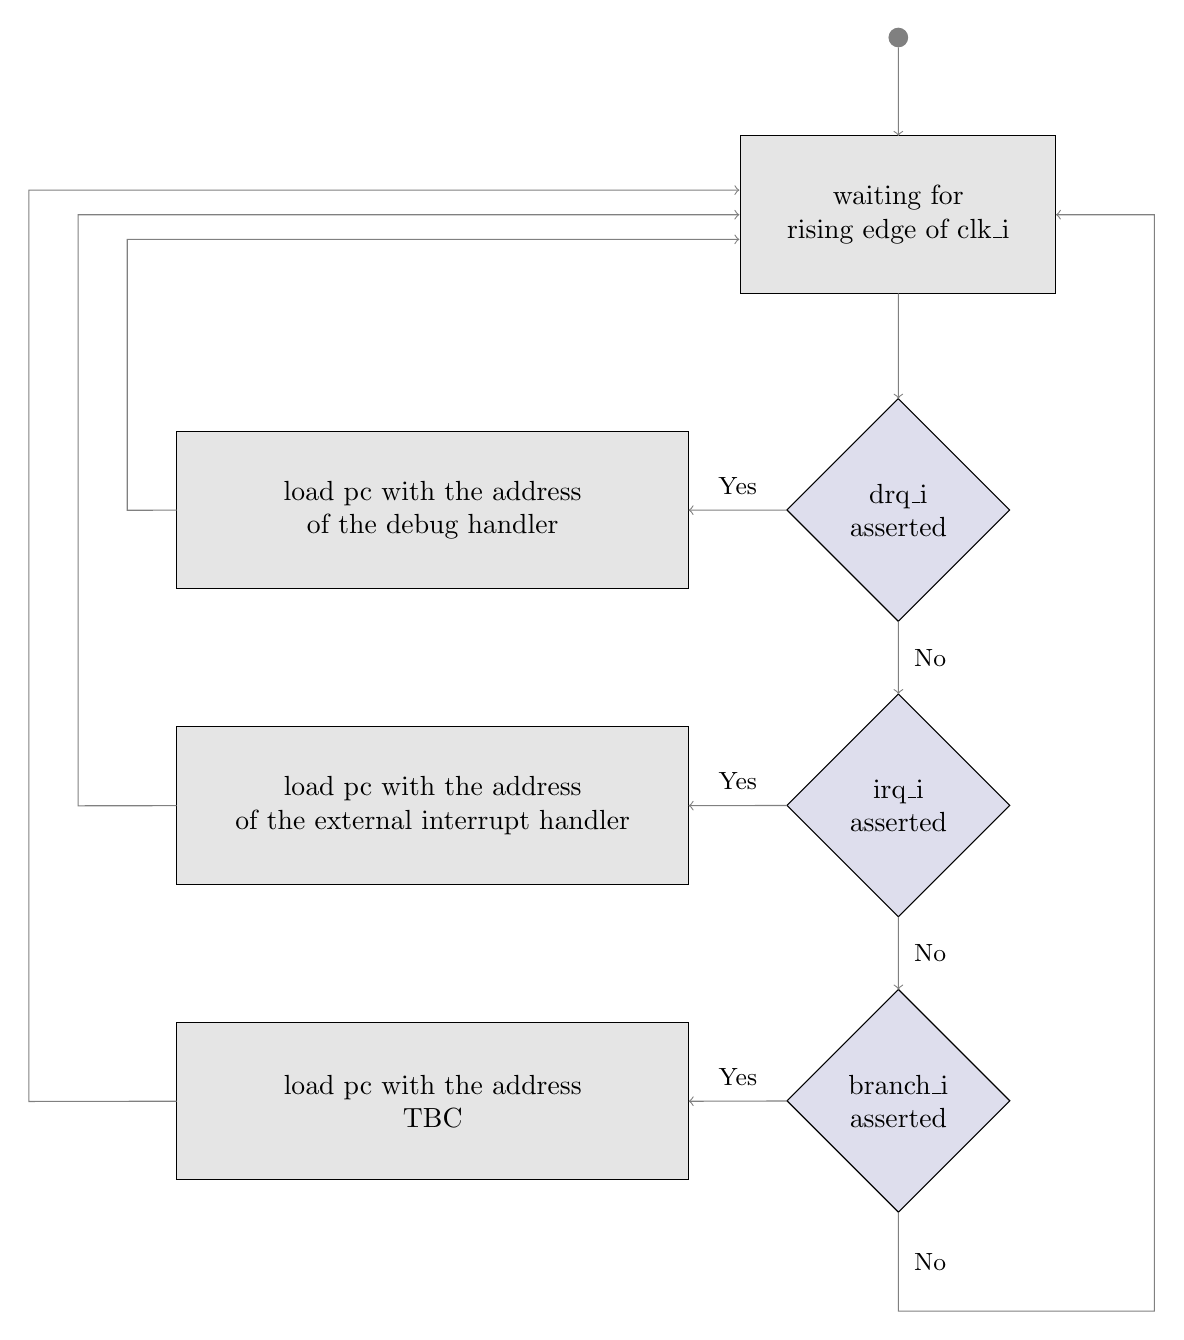
\begin{tikzpicture}[scale=1.25, draw=gray, inner sep=0, outer sep=0]
  \node[rectangle, draw=black,
    align=center,
    anchor=north west,
    minimum height = 2cm,
    minimum width = 4cm,
    fill = gray!20] (box1) at (0, 0) {waiting for\\rising edge of clk\_i};

  \node[rectangle, draw=black,
    minimum height = 2cm,
    minimum width = 2cm,
    rotate=45,
    fill = blue!30!gray!20] (if1) at ([yshift=-3cm]box1.center) {};
  \node[align=center] (if1-text) at (if1.center) {drq\_i\\asserted};

  \node[rectangle, draw=black,
    align=center,
    anchor=east,
    minimum height = 2cm,
    minimum width = 6.5cm,
    fill = gray!20] (box2) at ([xshift=-1cm]if1.north west) {load pc with the address \\ of the debug handler};

  \node[rectangle, draw=black,
    minimum height = 2cm,
    minimum width = 2cm,
    rotate=45,
    fill = blue!30!gray!20] (if2) at ([yshift=-3cm]if1.center) {};
  \node[align=center] (if2-text) at (if2.center) {irq\_i\\asserted};

  \node[rectangle, draw=black,
    align=center,
    anchor=east,
    minimum height = 2cm,
    minimum width = 6.5cm,
    fill = gray!20] (box3) at ([xshift=-1cm]if2.north west) {load pc with the address \\ of the external interrupt handler};

  \node[rectangle, draw=black,
    minimum height = 2cm,
    minimum width = 2cm,
    rotate=45,
    fill = blue!30!gray!20] (if3) at ([yshift=-3cm]if2.center) {};
  \node[align=center] (if3-text) at (if3.center) {branch\_i\\asserted};

  \node[rectangle, draw=black,
    align=center,
    anchor=east,
    minimum height = 2cm,
    minimum width = 6.5cm,
    fill = gray!20] (box4) at ([xshift=-1cm]if3.north west) {load pc with the address \\ TBC};

  \draw[->] (box1.south) -- (if1.north east);
  \draw[->] (if1.south west) -- node[right=0.2cm]{\small No} (if2.north east);
  \draw[->] (if2.south west) -- node[right=0.2cm]{\small No} (if3.north east);

  \draw[->] (if1.north west) -- node[above=0.2cm]{\small Yes} (box2.east);
  \draw[->] (if2.north west) -- node[above=0.2cm]{\small Yes} (box3.east);
  \draw[->] (if3.north west) -- node[above=0.2cm]{\small Yes} (box4.east);

  \node (cross1) at ([yshift=-1cm]if3.south west) {};
  \node (cross2) at ([xshift=1cm]box1.east) {};
  \draw[->] (if3.south west) -- node[right=0.2cm]{\small No} (if3.south west |- cross1.center) -- (cross1.center -| cross2.center) -- (cross2.center) -- (box1.east);

  \node (cross3) at ([xshift=-0.5cm]box2.west) {};
  \node (cross4) at ([xshift=-1cm]box3.west) {};
  \node (cross5) at ([xshift=-1.5cm]box4.west) {};

  \node (cross6) at ([yshift=-0.25cm]box1.west) {};
  \node (cross7) at (box1.west) {};
  \node (cross8) at ([yshift=0.25cm]box1.west) {};

  \draw[->] (box2.west) -- (cross3.center) -- (cross3.center |- cross6.west) -- (cross6.west);
  \draw[->] (box3.west) -- (cross4.center) -- (cross4.center |- cross7.west) -- (cross7.west);
  \draw[->] (box4.west) -- (cross5.center) -- (cross5.center |- cross8.west) -- (cross8.west);

  \node [circle, fill=gray, minimum height = 0.25cm, minimum width = 0.25cm] (start) at ([yshift=1cm]box1.north) {};
  \draw[->] (start.south) -- (box1.north) {};
\end{tikzpicture}
}

    \caption{Activity diagram of the jump logic behavior}
    \label{fig:jump-logic-behavior}
\end{figure}

\begin{figure}[H]
    \centering
    \begin{tikztimingtable}[%
    scale=0.9,
    timing/dslope=0.1,
    timing/.style={x=5ex,y=3ex},
    x=5ex,
    timing/rowdist=5ex,
    timing/name/.style={font=\footnotesize},
    timing/u/background/.style={fill=gray!20},
    timing/e/background/.style={fill=gray!20},
]

clk\_i & H 3{C C} L \\
npc\_o & 2U 2D{new pc value} 4U  \\
pc\_load\_o & 2L 0.2E 1.8H 0.2E 4L \\
pc & 4D{previous pc value} 4D{new pc value} \\
\extracode
% grid
\begin{pgfonlayer}{background}
\begin{scope}[semitransparent ,semithick]
\vertlines[darkgray,dotted]{2, 4, 6}
\end{scope}
\end{pgfonlayer}
\end{tikztimingtable}

    \caption{Timing diagram for the output port of the jump logic.}
    \label{fig:jump-logic-output}
\end{figure}

\subsection{PC register}

\subsection{Wishbone master}

\begin{figure}[H]
    \centering
    \vspace{1em}
\scalebox{0.85}{
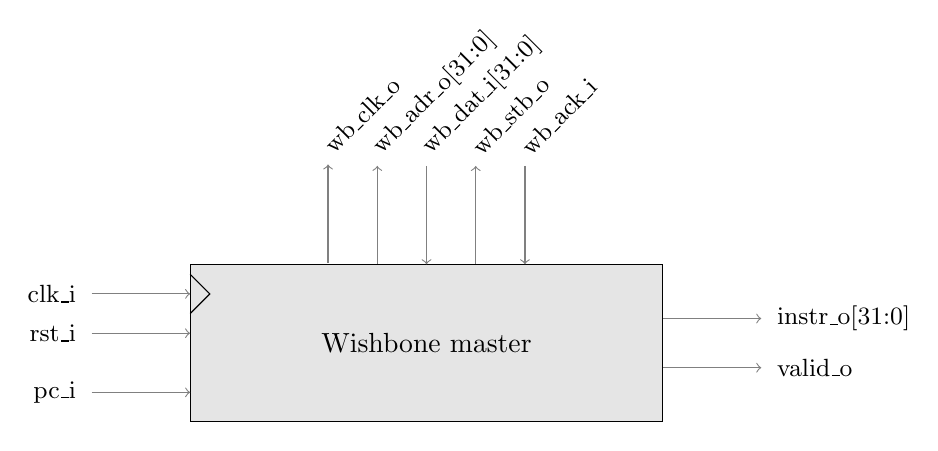
\begin{tikzpicture}[scale=1.25, draw=gray, inner sep=0, outer sep=0]
  \node[rectangle, draw=black,
    anchor=south,
    align=center,
    minimum height = 2cm,
    minimum width = 6cm,
    fill = gray!20] (mem) at (0, 0) {Wishbone master};

  \node(uport4) at ([xshift=0.5cm]mem.north) {};
  \node(uport3) at ([xshift=-0.5cm]uport4.center) {};
  \node(uport2) at ([xshift=-0.5cm]uport3.center) {};
  \node(uport1) at ([xshift=-0.5cm]uport2.north) {};
  \node(uport5) at ([xshift=0.5cm]uport4.center) {};
  \draw[<-] ([yshift=1cm]uport1.center) node[above=0.2cm, anchor=west, rotate=45]{\small wb\_clk\_o} -- (uport1.center);
  \draw[<-] ([yshift=1cm]uport2.center) node[above=0.2cm, anchor=west, rotate=45]{\small wb\_adr\_o[31:0]} -- (uport2.center);
  \draw[->] ([yshift=1cm]uport3.center) node[above=0.2cm, anchor=west, rotate=45]{\small wb\_dat\_i[31:0]} -- (uport3.center);
  \draw[<-] ([yshift=1cm]uport4.center) node[above=0.2cm, anchor=west, rotate=45]{\small wb\_stb\_o} -- (uport4.center);
  \draw[->] ([yshift=1cm]uport5.center) node[above=0.2cm, anchor=west, rotate=45]{\small wb\_ack\_i} -- (uport5.center);

  \node(lport1) at ([yshift=-0.5cm]mem.west) {};
  \draw[->] ([xshift=-1cm]lport1.center) node[left=0.2cm, anchor=east]{\small pc\_i} -- (lport1.center);

  \node(rport1) at ([yshift=0.25cm]mem.east) {};
  \node(rport2) at ([yshift=-0.5cm]rport1.center) {};
  \draw[<-] ([xshift=1cm]rport1.center) node[right=0.2cm, anchor=west]{\small instr\_o[31:0]} -- (rport1.center);
  \draw[<-] ([xshift=1cm]rport2.center) node[right=0.2cm, anchor=west]{\small valid\_o} -- (rport2.center);

  \node (clk) at ([yshift=-0.3cm]mem.north west) {};
  \draw[->] ([xshift=-1cm]clk.center) node[left=0.2cm, anchor=east]{\small clk\_i} -- (clk.center);
  % clk triangle
  \draw[-, draw=black] ([yshift=0.2cm]clk.center) -- ([xshift=0.2cm]clk.center) -- ([yshift=-0.2cm]clk.center);

  \node (rst) at ([yshift=-0.4cm]clk.center) {};
  \draw[->] ([xshift=-1cm]rst.center) node[left=0.2cm, anchor=east]{\small rst\_i} -- (rst.center);
\end{tikzpicture}
}

    \caption{Schematic view of the interface of the Wishbone Master}
    \label{fig:ifm-wishbone-master}
\end{figure}

\begin{content}
  The wishbone master fetches from memory the instruction to be executed. Its interface is described in table \ref{tab:ifm-wishbone-master}.
\end{content}

{
  \vspace{0.5em}
  \begin{center}
    \refstepcounter{table}
    Table \thetable: Instruction Fetch Module interface signals\label{tab:ifm-wishbone-master}
  \end{center}

\footnotesize
\begin{xltabular}{0.9\textwidth}{|l|c|c|X|}
  \hline
  \cellcolor{gray!20}\textbf{NAME} & \cellcolor{gray!20}\textbf{TYPE} & \cellcolor{gray!20}\textbf{WIDTH} & \cellcolor{gray!20}\textbf{DESCRIPTION} \\
  \hline
  clk\_i & I & 1 & Clock input. \\
  \hline
  rst\_i & I & 1 & Reset input. \\
  \hline
  \multicolumn{4}{|l|}{\textbf{WISHBONE MASTER}} \\
  \hline
  wb\_clk\_o & O & 1 & Wishbone clock output. This is hardwired to clk\_i. \\
  \hline
  wb\_adr\_o & O & 32 & Wishbone read address.  \\
  \hline
  wb\_dat\_i & I & 32 & Wishbone read data. \\
  \hline
  wb\_stb\_o & O & 1 & Strobe output indicates a valid data transfer cycle. \\
  \hline
  wb\_ack\_i & I & 1 & Acknowledge. Indicates a normal termination of a bus cycle. \\
  \hline
  \multicolumn{4}{|l|}{\textbf{OUTPUT}} \\
  \hline
  instr\_o & O & 32 & Instruction to be executed. \\
  \hline
  valid\_o & O & 1 & Asserted when the instruction output is valid. \\
  \hline
\end{xltabular}
}


\subsection{Output logic}

\newpage
\section{Decode Module}
\newpage

\section{Register Module}

\begin{figure}[h!]
    \centering
    \vspace{1em}
\scalebox{0.85}{
\begin{tikzpicture}[scale=1.25, draw=gray, inner sep=0, outer sep=0]
  \node[rectangle, draw=white,
    align=center,
    minimum height = 4.75cm,
    minimum width = 4cm,
    fill = white] (back) at (6, 2.5) {Block RAM \\ \small DP16KD};
  \node[rectangle, draw=black,
    align=center,
    anchor=south,
    minimum height = 4cm,
    minimum width = 4cm,
    fill = blue!30!gray!20] (BRAM) at (back.south) {Block RAM \\ \small DP16KD};

  \node[rectangle, draw=black,
    align=center,
    anchor=east,
    minimum height = 4cm,
    minimum width = 1.5cm,
    fill = gray!20] (glue1) at ([xshift=-0.5cm]BRAM.west) {};
  \node[rotate=90] (glue1text) at (glue1.center) {Read logic};

  \node[rectangle, draw=black,
    align=center,
    anchor=west,
    minimum height = 4cm,
    minimum width = 1.5cm,
    fill = gray!20] (glue2) at ([xshift=0.5cm]BRAM.east) {};
  \node[rotate=90] (glue2text) at (glue2.center) {Write logic};

  \node[dashed, draw=black, align=center, inner sep=1cm, fit=(BRAM) (back) (glue1) (glue2)] (border) {};
  \node[anchor=north west, inner sep=0.25cm] (border-text) at (border.north west) {REGM};

  \node (lport2) at ([yshift=0.5cm]glue1.west) {};
  \node (lport1) at ([yshift=0.5cm]lport2.center) {};
  \draw[->] ([xshift=-1.5cm]lport1.center) node[left=0.2cm, anchor=east]{\small raddr1\_i[4:0]} -- (lport1.center);
  \draw[<-] ([xshift=-1.5cm]lport2.center) node[left=0.2cm, anchor=east]{\small rdata1\_o[31:0]} -- (lport2.center);

  \node (lport3) at ([yshift=-0.5cm]glue1.west) {};
  \node (lport4) at ([yshift=-0.5cm]lport3.west) {};
  \draw[->] ([xshift=-1.5cm]lport3.center) node[left=0.2cm, anchor=east]{\small raddr2\_i[4:0]} -- (lport3.center);
  \draw[<-] ([xshift=-1.5cm]lport4.center) node[left=0.2cm, anchor=east]{\small rdata2\_o[31:0]} -- (lport4.center);

  \node (rport2) at (glue2.east) {};
  \node (rport1) at ([yshift=0.5cm]rport2.center) {};
  \node (rport3) at ([yshift=-0.5cm]rport2.center) {};
  \draw[->] ([xshift=1.5cm]rport1.center) node[right=0.2cm, anchor=west]{\small waddr\_i[4:0]} -- (rport1.center);
  \draw[->] ([xshift=1.5cm]rport2.center) node[right=0.2cm, anchor=west]{\small write\_i} -- (rport2.center);
  \draw[->] ([xshift=1.5cm]rport3.center) node[right=0.2cm, anchor=west]{\small wdata\_i[31:0]} -- (rport3.center);

  \node (clk) at ([yshift=-1cm]border.north west) {};
  \draw[->] ([xshift=-1.5cm]lport3.center |- clk.center) node[left=0.2cm, anchor=east]{\small clk\_i} -- (clk.center);
  % clk triangle
  \draw[-, dashed, draw=black] ([yshift=0.25cm]clk.center) -- ([xshift=0.25cm]clk.center) -- ([yshift=-0.25cm]clk.center);

  \draw[<->] (glue1.east) -- (BRAM.west);
  \draw[<->] (glue2.west) -- (BRAM.east);
\end{tikzpicture}
}

    \caption{Schematic view of the Register Module}
    \label{fig:regm}
\end{figure}

\begin{content}
The register module implements the 32 internal registers of ECAP5-DPROC. It has two reading port and one writing port. The signals are described in table \ref{tab:regm-interface}. 
\end{content}

\begin{table}[H]
  \centering
  {
\footnotesize
\begin{tabularx}{0.9\textwidth}{|l|c|c|X|}
  \hline
  \cellcolor{gray!20}\textbf{NAME} & \cellcolor{gray!20}\textbf{TYPE} & \cellcolor{gray!20}\textbf{WIDTH} & \cellcolor{gray!20}\textbf{DESCRIPTION} \\
  \hline
  clk\_i & I & 1 & Clock input. \\
  \hline
  \multicolumn{4}{|l|}{\textbf{FIRST READING PORT}} \\
  \hline
  raddr1\_i & I & 5 & Register selector. \\
  \hline
  rdata1\_o & O & 32 & Selected register value. \\
  \hline
  \multicolumn{4}{|l|}{\textbf{SECOND READING PORT}} \\
  \hline
  raddr2\_i & I & 5 & Register selector. \\
  \hline
  rdata2\_o & O & 32 & Selected register value. \\
  \hline
  \multicolumn{4}{|l|}{\textbf{WRITING PORT}} \\
  \hline
  waddr\_i & I & 5 & Register selector. \\
  \hline
  write\_i & I & 1 & Asserted to indicate a write. \\
  \hline
  wdata\_i & I & 32 & Data to be written. \\
  \hline
\end{tabularx}
}

  \caption{Register Module interface signals}
  \label{tab:regm-interface}
\end{table}

\begin{content}
  When reading, \texttt{rdata1\_i} and \texttt{rdata2\_i} output, on the rising edge of \texttt{clk\_i}, the value of the register respectively selected by \texttt{raddr1\_i} and \texttt{raddr2\_i}. A register write happens on the rising edge of \texttt{clk\_i} when \texttt{write\_i} is asserted, writing the value \texttt{wdata\_i} in the register selected by \texttt{waddr\_i}.
\end{content}

\newpage

\section{Execute Module}
\newpage

\section{Write-Back Module}
\newpage

\section{Debug}
\newpage
